\documentclass[a4paper]{article}
\usepackage[spanish]{babel}
\usepackage[utf8]{inputenc}
\usepackage{algorithm}
\usepackage{algpseudocode}
\usepackage{graphicx}
\graphicspath{ {images/} }

\begin{document}

\title{Sorting}
\author{Fer Frassia}
\maketitle
\tableofcontents

\newpage
\section{Selection Sort}

\subsection{C\'odigo:}
\begin{algorithm}
\caption{Selection Sort}\label{selection}
\begin{algorithmic}[1]
\Procedure{selectionSort}{$A$}
   \For{\textbf{$i \gets 1$ to} $length(A)$}
   	\State $min \gets selectMin(A, i)$ \Comment{selects min index from A[i..n]}
	\State $swap A[i] \leftrightarrow A[min]$ 
    \EndFor
\EndProcedure
\end{algorithmic}
\end{algorithm}

\subsection{Invariante:}
\begin{itemize}
	\item{A[1..i-1] son los m\'as chicos y est\'an ordenados}
	\item{A[i..n] son los m\'as grandes}
\end{itemize}

\subsection{Peor caso: $\Theta (n^{2})$ - indedependiente al orden inicial}
\subsection{Mejor caso: $\Theta (n^{2})$ - independiente al orden inicial}
\subsection{Estable: S\'i}
\subsection{In place: S\'i}
\subsection{Swaps: $\Theta (n)$}
\subsection{Si se corta, da un subarreglo ordenado: S\'i, la parte baja}
\subsection{Insertar elementos en runtime: No}
	
\newpage
\section{Insertion Sort}

\subsection{C\'odigo:}
\begin{algorithm}
\caption{Insertion Sort}\label{selection}
\begin{algorithmic}[1]
\Procedure{insertionSort}{$A$}
   \For{\textbf{$i \gets 1$ to} $length(A)$}
   	\State $key \gets A[i]$
	\State $j \gets i-1$
    \While{$j > 0 \wedge A[j] > key$ }
    	\State $A[j+1] \gets A[j]$
	\State $j --$
    \EndWhile
    \State $A[j+1] \gets key$
    \EndFor
\EndProcedure
\end{algorithmic}
\end{algorithm}

\subsection{Invariante:}
\begin{itemize}
	\item{A[1..i-1] son los originales y est\'an relativamente ordenados}
\end{itemize}

\subsection{Peor caso: $\mathcal{O}(n^{2})$ - orden inverso}
\subsection{Mejor caso: $\mathcal{O}(n)$ - ordenado}
\subsection{Estable: S\'i}
\subsection{In place: S\'i}
\subsection{Swaps: $\mathcal{O}(n^{2})$ - peor caso}
\subsection{Si se corta, da un subarreglo ordenado: No, pero da orden parcial relativo}
\subsection{Insertar elementos en runtime: S\'i}

\newpage
\section{Bubble Sort}

\subsection{C\'odigo:}
\begin{algorithm}
\caption{Bubble Sort}\label{selection}
\begin{algorithmic}[1]
\Procedure{bubbleSort}{$A$}
   \For{\textbf{$i \gets 1$ to} $length(A)$}
   	\For{\textbf{$j \gets 1$ to} $length(A)-i$}
		\If{$A[j] > A[j+1]$}
			\State $swap A[j] \leftrightarrow A[j+1]$
		\EndIf
	\EndFor
    \EndFor
\EndProcedure
\end{algorithmic}
\end{algorithm}

\subsection{Invariante:}
\begin{itemize}
	\item{A[n-i..n] est\'an ordenados}
\end{itemize}

\subsection{Peor caso: $\mathcal{O}(n^{2})$}
\subsection{Mejor caso: $\mathcal{O}(n)$ - ordenado y con chequeo de swap}
\subsection{Estable: S\'i}
\subsection{In place: S\'i}
\subsection{Swaps: $\mathcal{O}(n^{2})$ - peor caso}
\subsection{Si se corta, da un subarreglo ordenado: S\'i, la parte alta}
\subsection{Insertar elementos en runtime: S\'i, pero los insert\'as adelante}

\newpage
\section{HeapSort}

\subsection{C\'odigo:}
\begin{algorithm}
\caption{Heap Sort}\label{selection}
\begin{algorithmic}[1]
\Procedure{heapSort}{$A$}
	\State $buildMaxHeap(A)$
	\For{\textbf{$i \gets length(A)$ downTo} $2$}
		\State $swap A[1] \leftrightarrow A[i]$
		\State $heapSize(A)--$
		\State $maxHeapify(A,1)$
	\EndFor
\EndProcedure
\end{algorithmic}
\end{algorithm}

\subsection{Invariante:}
\begin{itemize}
	\item{A[1..i] es maxHeap y contiene los i elementos m\'as chicos.}
	\item{A[i+1..n] contiene los n-i elementos m\'as grandes, ordenados (en su posici\'on final).}
\end{itemize}

\subsection{Peor caso: $\Theta (n \log{} n)$ - independiente al orden inicial}
\subsection{Mejor caso: $\Theta (n \log{} n)$ - independiente al orden inicial}
\subsection{Estable: No}
\subsection{In place: S\'i}
\subsection{Si se corta, da un subarreglo ordenado: S\'i, la parte alta}
\subsection{Insertar elementos en runtime: No}

\newpage
\section{QuickSort}

\subsection{C\'odigo:}
\begin{algorithm}
\caption{Quick Sort}\label{selection}
\begin{algorithmic}[1]
\Procedure{quickSort}{$A, p, r$}
	\If{$p < r$}
		\State $q \gets partition(A,p,r)$
		\State $quickSort(A,p,q-1)$
		\State $quickSort(A,q+1,r)$
	\EndIf
\EndProcedure
\end{algorithmic}
\end{algorithm}

\begin{algorithm}
\caption{Partition}\label{selection}
\begin{algorithmic}[1]
\Procedure{partition}{$A, p, r$}
	\State $x \gets A[r]$
	\State $i \gets p-1$
	\For{\textbf{$ j \gets p $ to} $r-1$}
		\If{$A[j] \leq x$}
			\State $i++$
			\State $swap A[i] \leftrightarrow A[j]$
		\EndIf
	\EndFor
	\State $swap A[i+1] \leftrightarrow A[r]$
	\State \textbf{return} $i+1$
\EndProcedure
\end{algorithmic}
\end{algorithm}

\subsection{Correctitud de QuickSort:}
Inducci\'on global sobre n 

\subsection{Invariante de Partition:}
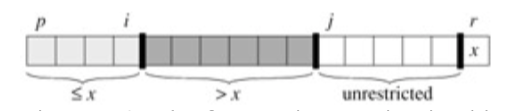
\includegraphics[width=1\textwidth]{invPartition}

\subsection{Peor caso: $\mathcal{O}(n^{2})$ - orden, orden inverso, todos iguales}
\subsection{Mejor caso: $\mathcal{O}(n \log{}n)$}
\subsection{Promedio: $\mathcal{O}(n \log{}n)$}
\subsection{Estable: No}
\subsection{In place: S\'i}
\subsection{Swaps: $\mathcal{O}(n^{2})$ - peor caso}
\subsection{Si se corta, da un subarreglo ordenado: No}
\subsection{Insertar elementos en runtime: No}

\newpage
\section{MergeSort}

\subsection{C\'odigo:}
\begin{algorithm}
\caption{Merge Sort}\label{selection}
\begin{algorithmic}[1]
\Procedure{mergeSort}{$A, l, u$}
	\If{$l < u$}
		\State $m \gets (l+u)/2)$
		\State $mergeSort(A,l,m)$
		\State $mergeSort(A,m+1,u)$
		\State $merge(A,l,m,u)$
	\EndIf
\EndProcedure
\end{algorithmic}
\end{algorithm}

\subsection{Correctitud de mergeSort:}
Inducci\'on global sobre n 

\subsection{Peor caso: $\mathcal{O}(n \log{}n)$}
\subsection{Mejor caso: $\mathcal{O}(n \log{}n)$}
\subsection{Promedio: $\mathcal{O}(n \log{}n)$}
\subsection{Estable: S\'i}
\subsection{In place: S\'i (aunque com\'unmente no)}
\subsection{Si se corta, da un subarreglo ordenado: No}
\subsection{Insertar elementos en runtime: No}

\newpage
\section{Counting Sort}

\subsection{C\'odigo:}
\begin{algorithm}
\caption{Counting Sort}\label{selection}
\begin{algorithmic}[1]
\Procedure{countingSort}{$A,k$}
	\State $B \gets [0,..,0]$ \Comment{arreglo de k+1 posiciones - $\mathcal{O}(k)$}
	\For{\textbf{$i \gets 1$ to} $length(A)$} \Comment{cuento apariciones - $\mathcal{O}(n)$}
		\State $B[A[i]]++$
	\EndFor
	\State $indexA \gets 1$
	\For{\textbf{$i \gets 1$ to} $length(B)$} \Comment{inserto cantidad de apariciones - $\mathcal{O}(n+k)$}
		\While{$B[i] > 0$} 
			\State $A[indexA] \gets i$
			\State $B[i]--$
			\State $indexA++$
		\EndWhile
	\EndFor
\EndProcedure
\end{algorithmic}
\end{algorithm}

\subsection{Invariante:}

\subsection{Peor caso:}
\subsection{Mejor caso:}
\subsection{Estable:}
\subsection{In place:}
\subsection{Swaps:}
\subsection{Si se corta, da un subarreglo ordenado:}
\subsection{Insertar elementos en runtime:}

\end{document}